\documentclass{ximera}
%% You can put user macros here
%% However, you cannot make new environments

\listfiles

\graphicspath{{./}{firstExample/}{secondExample/}}

\usepackage{tikz}
\usepackage{tkz-euclide}
\usepackage{tikz-3dplot}
\usepackage{tikz-cd}
\usetikzlibrary{shapes.geometric}
\usetikzlibrary{arrows}
\usetkzobj{all}
\pgfplotsset{compat=1.13} % prevents compile error.

%\renewcommand{\vec}[1]{\mathbf{#1}}
\renewcommand{\vec}{\mathbf}
\newcommand{\RR}{\mathbb{R}}
\newcommand{\dfn}{\textit}
\newcommand{\dotp}{\cdot}
\newcommand{\id}{\text{id}}
\newcommand\norm[1]{\left\lVert#1\right\rVert}
 
\newtheorem{general}{Generalization}
\newtheorem{initprob}{Exploration Problem}

\tikzstyle geometryDiagrams=[ultra thick,color=blue!50!black]

%\DefineVerbatimEnvironment{octave}{Verbatim}{numbers=left,frame=lines,label=Octave,labelposition=topline}



\usepackage{mathtools}


\title{Where was Eye? Part I} \license{CC BY-NC-SA 4.0}

\begin{document}

\begin{abstract}
\end{abstract}
\maketitle

\section*{Where was Eye? Part I}

\begin{exploration}\label{exp:matchPic}
Three students, Adam, Benjamin, and Cayla, took part in a photography competition.  All three submitted photos of railroad tracks.  Adam and Benjamin took photos from their natural height; Cayla flew a drone high above her head to take a picture.
    \begin{image}
         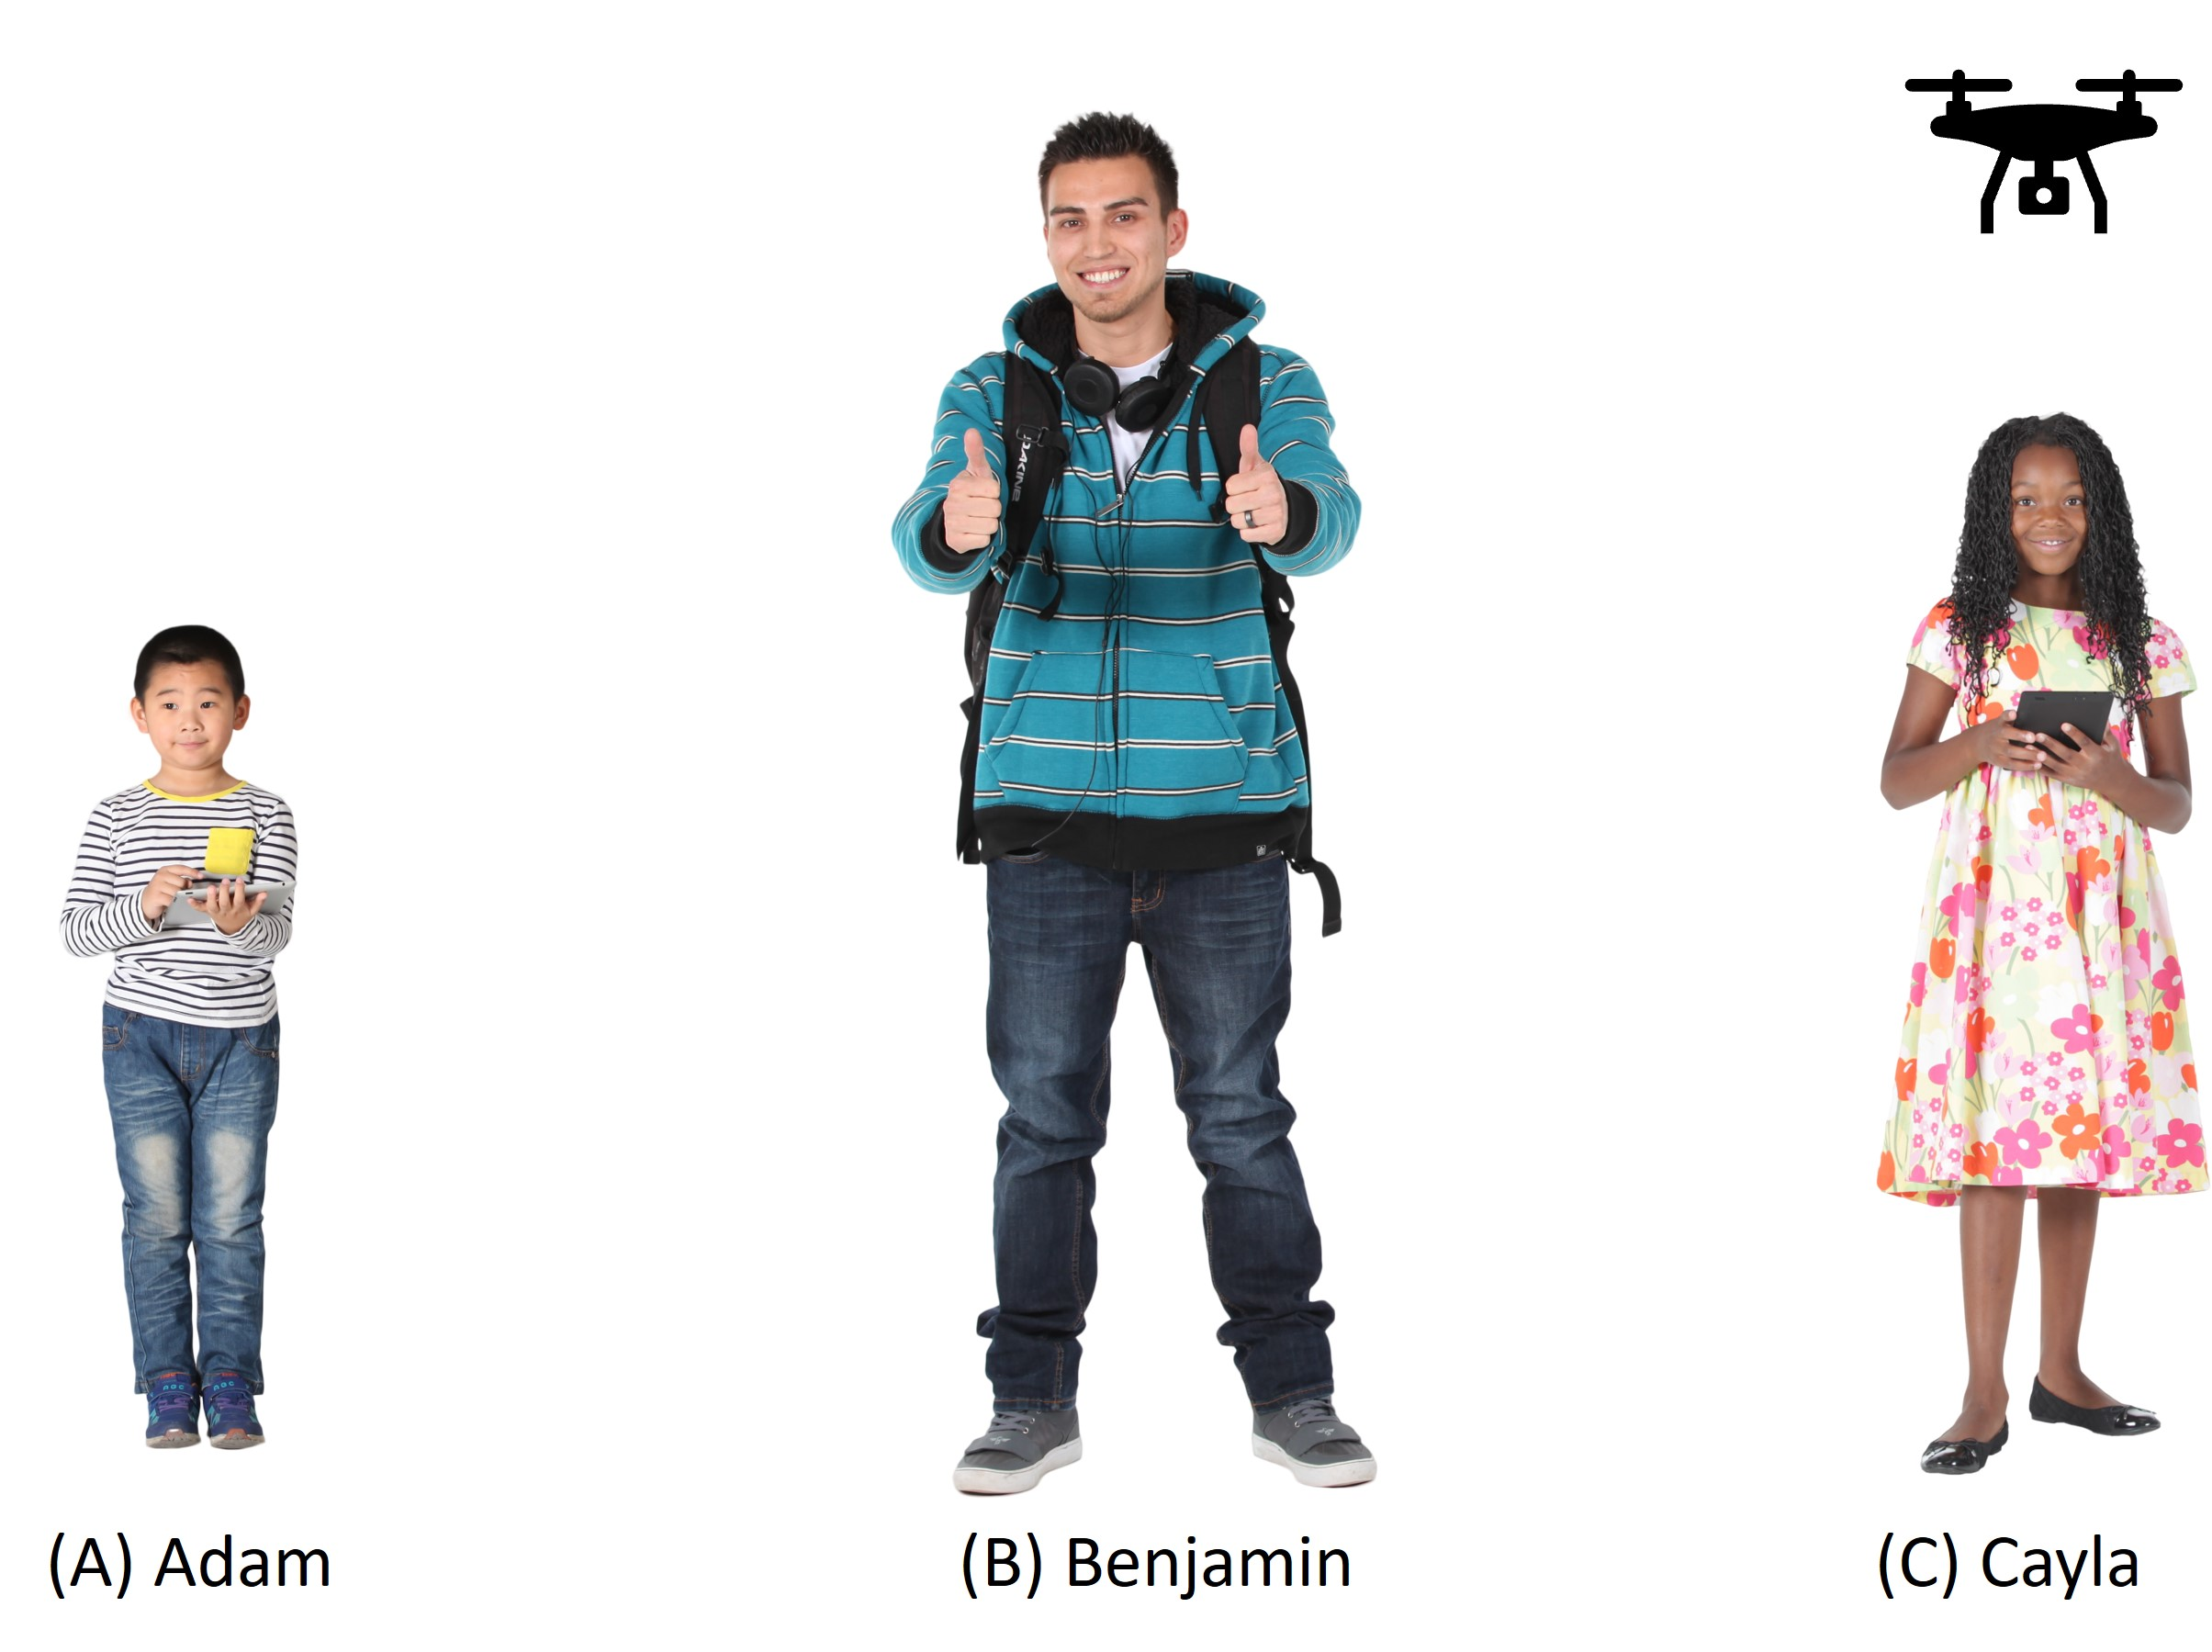
\includegraphics[width=5in]{AdamBenjaminCayla.jpg}
\end{image}
The images Adam, Benjamin, and Cayla took appear below (in no particular order).
\begin{image}
         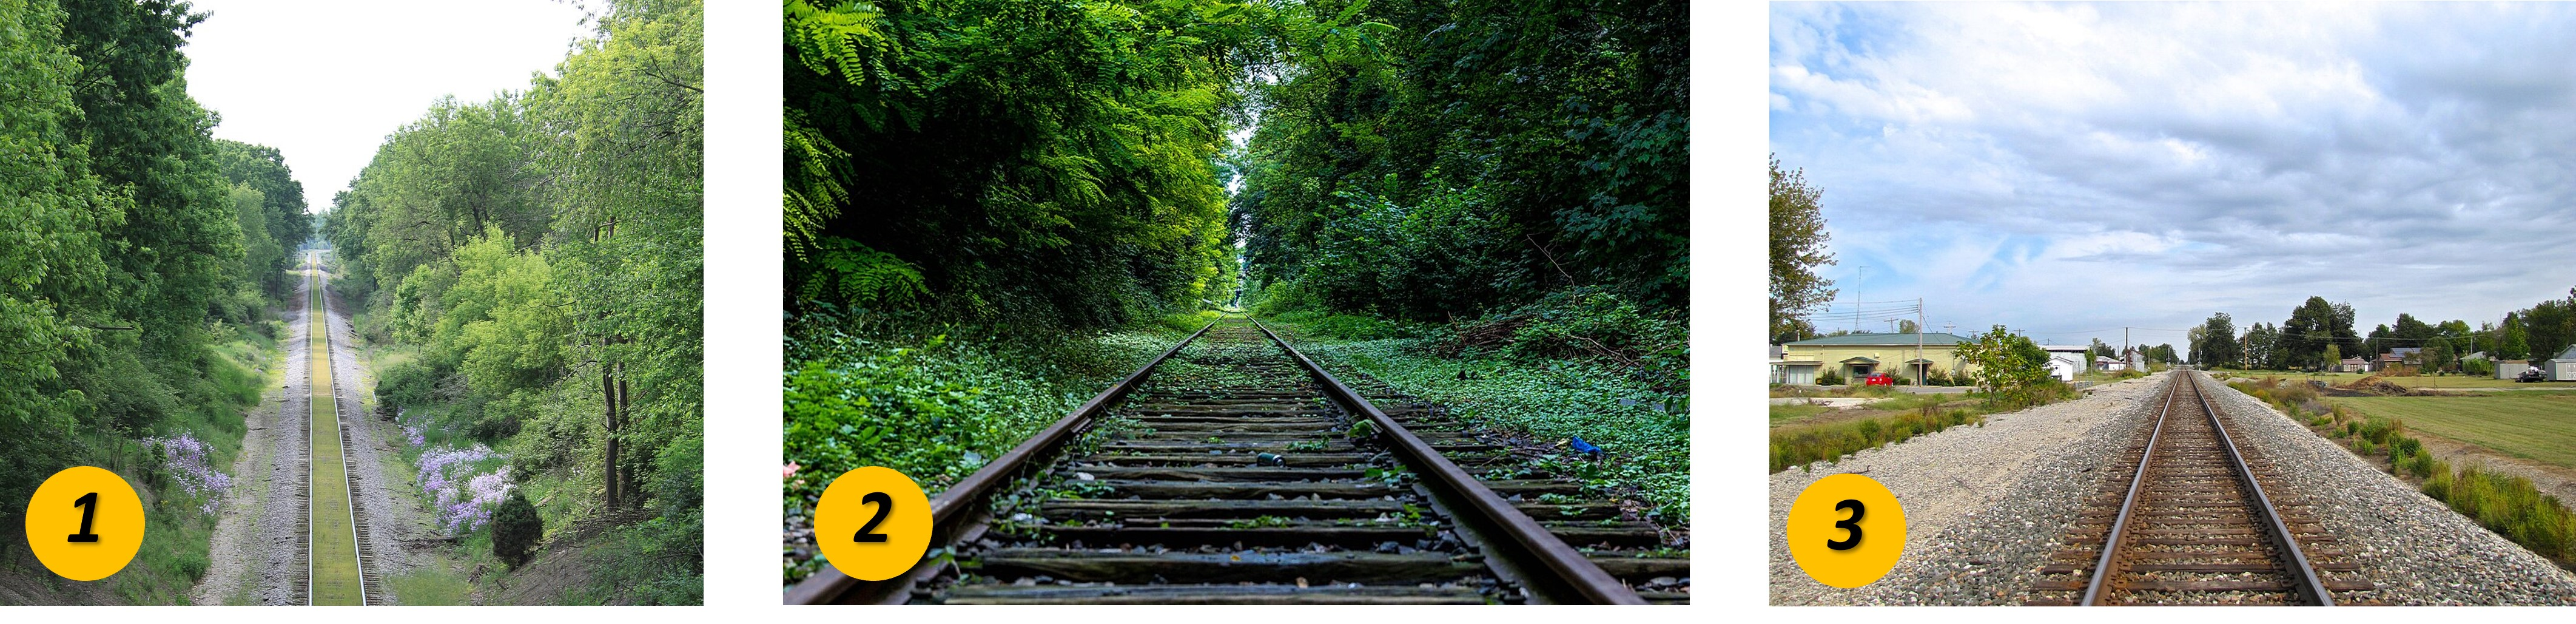
\includegraphics[width=5in]{threePics.jpg}
\end{image}
Match each image with the photographer who took it.

Photo 1 was taken by 
\begin{multipleChoice}
    \choice{Adam}
    \choice{Benjamin}
    \choice[correct]{Cayla}
\end{multipleChoice}

Photo 2 was taken by 
\begin{multipleChoice}
    \choice[correct]{Adam}
    \choice{Benjamin}
    \choice{Cayla}
\end{multipleChoice}

Photo 3 was taken by 
\begin{multipleChoice}
    \choice{Adam}
    \choice[correct]{Benjamin}
    \choice{Cayla}
\end{multipleChoice}

In small groups, discuss the reasons for your choices.  Do you think it is possible to use these photographs to estimate the height of the camera that took each photo?
\end{exploration}

\begin{exploration}\label{exp:trianglesAtBase}
    Let's look at the three pictures geometrically.  The rails appear to meet at a single point.  
    
\begin{image}
         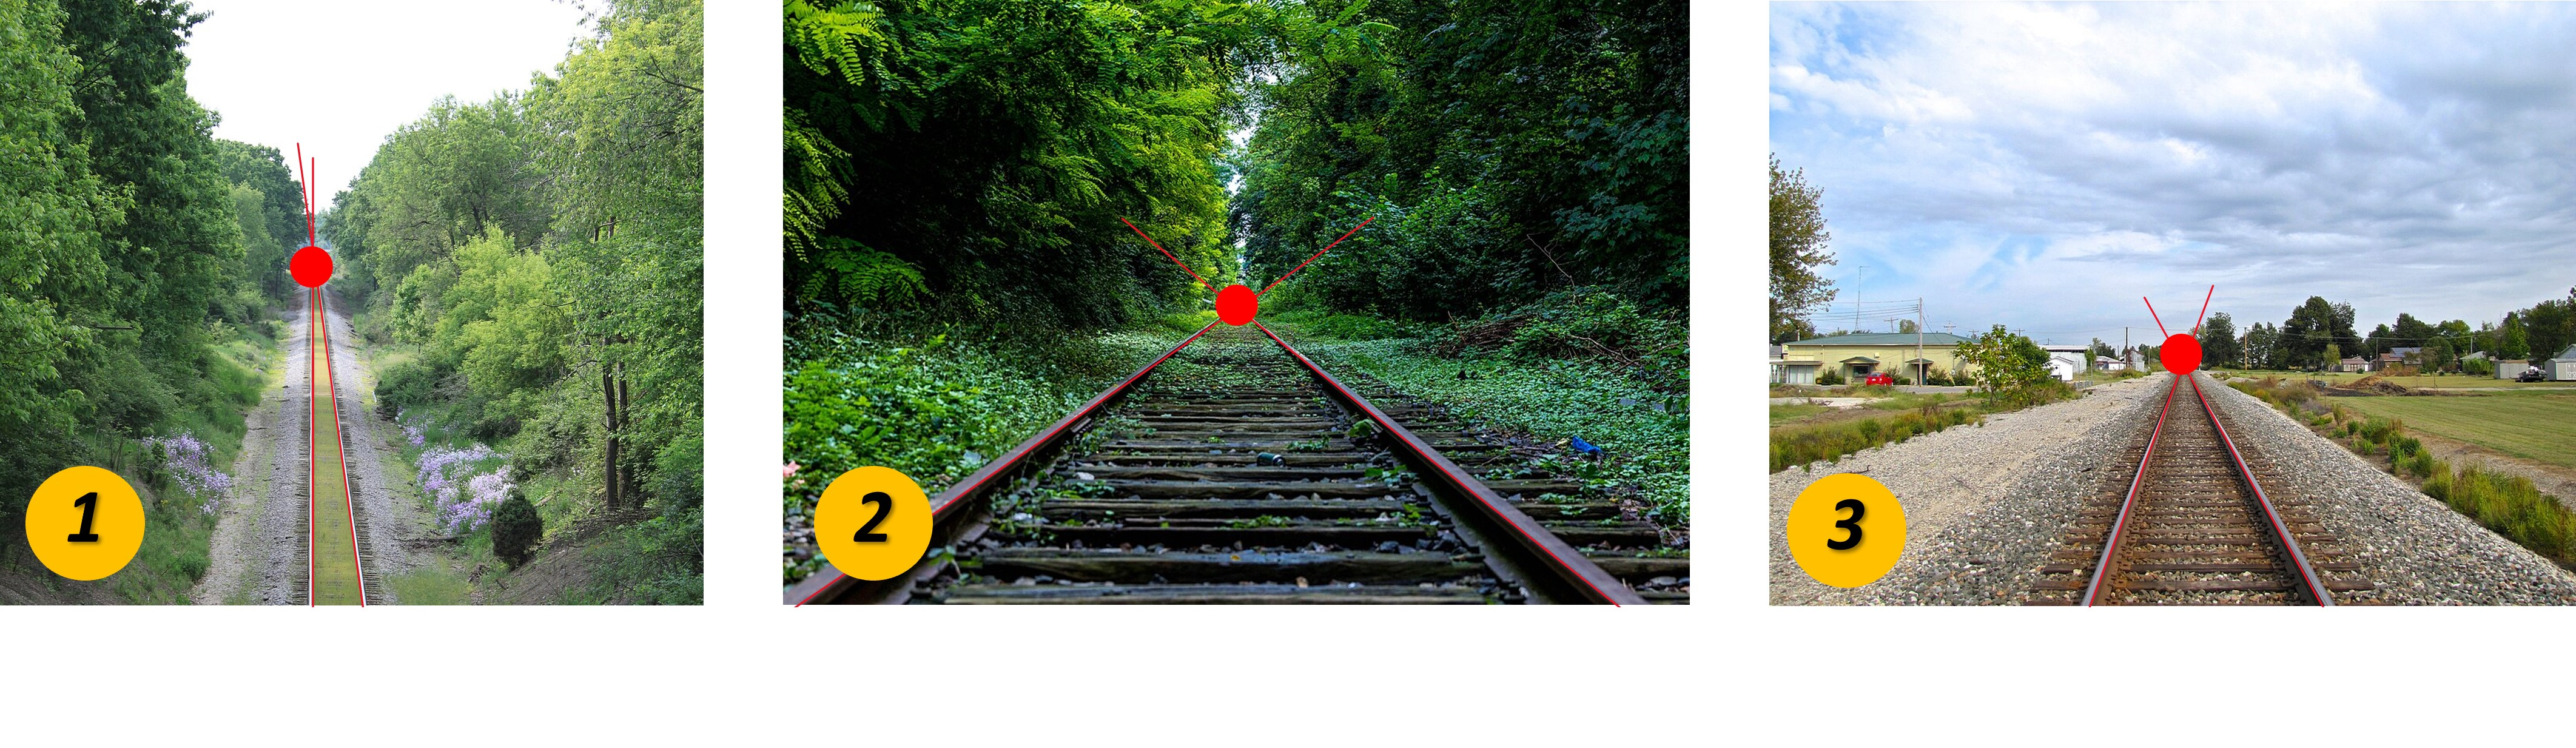
\includegraphics[width=5in]{vanishingPoint.jpg}
\end{image}
    
    Do you know what this point is called?
    \begin{multipleChoice}
        \choice{Center point}
        \choice[correct]{Vanishing point}
        \choice{Vertex}
        \choice{End point}
    \end{multipleChoice}

The rails, together with the bottom of each photo, form triangles.  

\begin{image}
         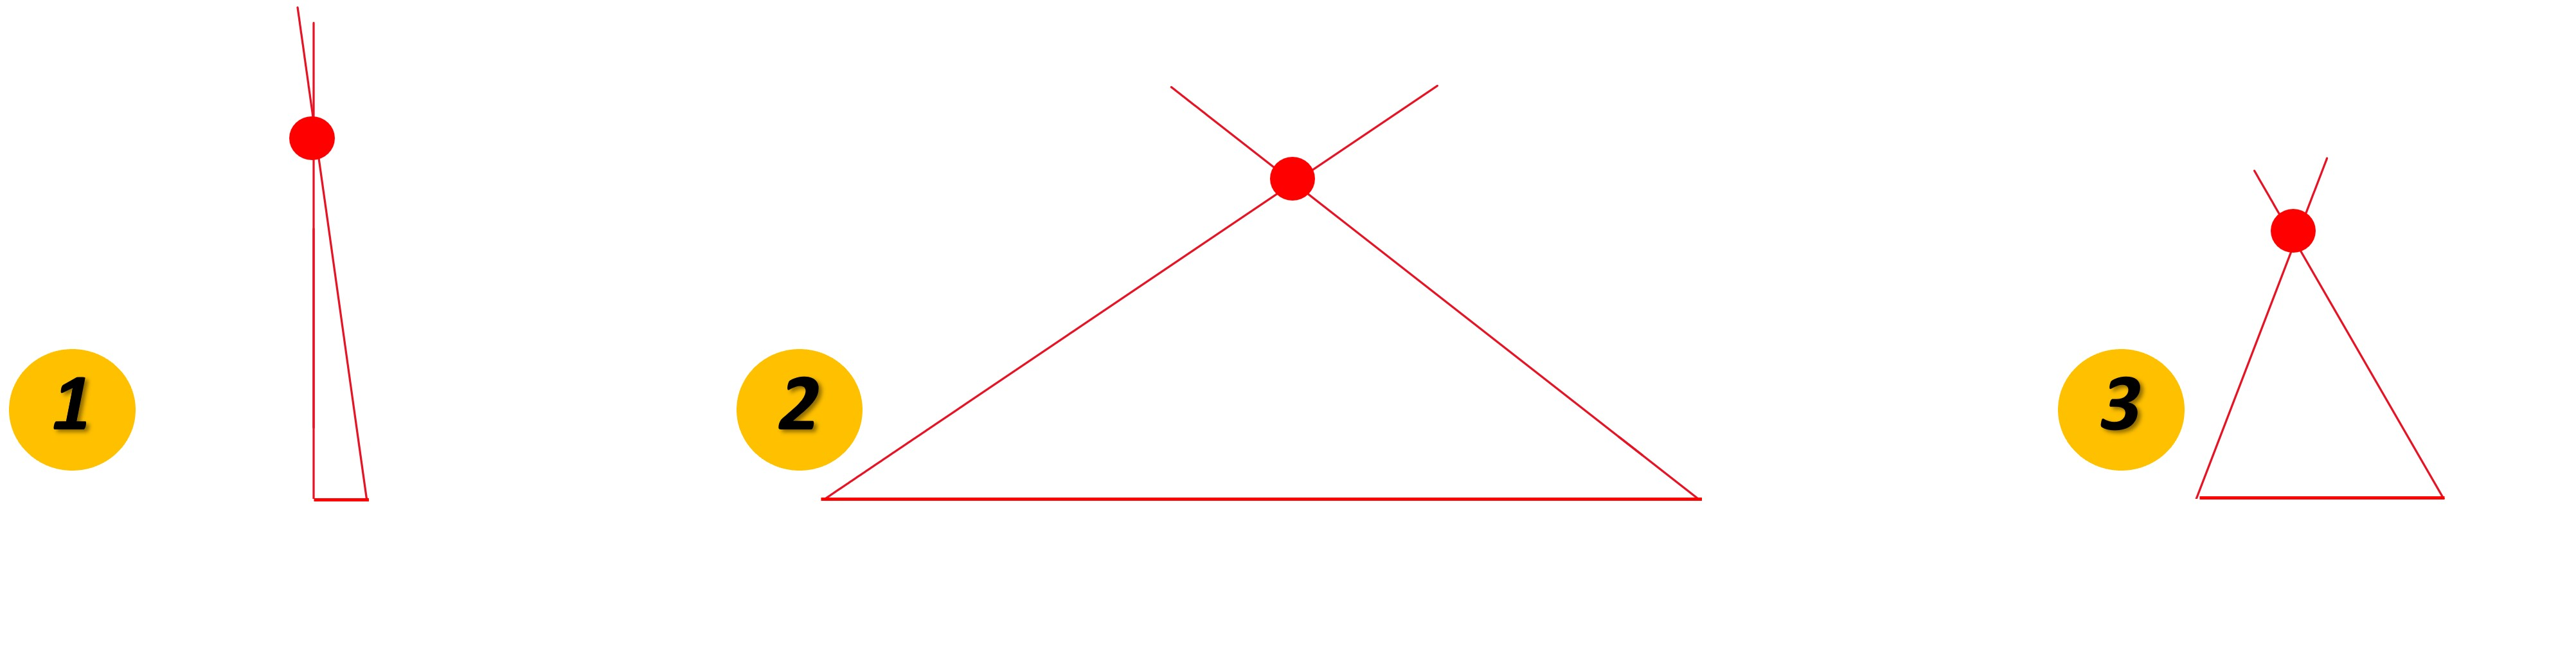
\includegraphics[width=5in]{triangles.jpg}
\end{image}

You might describe the first triangle as tall and narrow, and the second triangle as short and wide.  These descriptions refer to the \emph{proportions} of these triangles.  To really see the difference in the proportions, we can make the bases of the triangles the same size.  This makes sense to do because railroad tracks have the same width everywhere in the U.S.

\begin{image}
         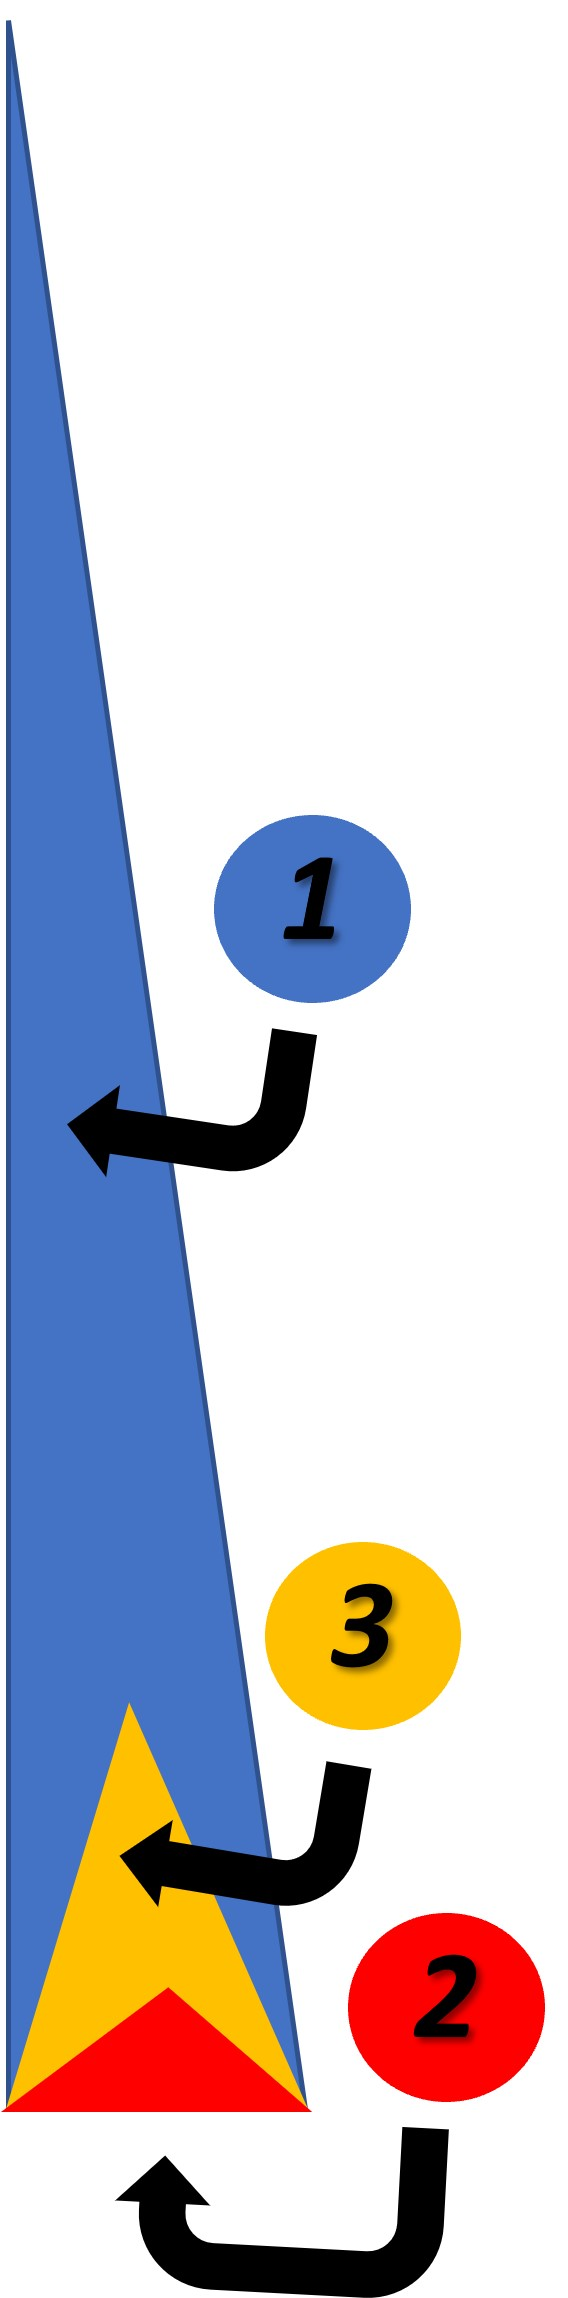
\includegraphics[width=3.5in]{matchedTriangles.jpg}
\end{image}

In groups, discuss the relationship between the height of the camera and the height of the triangles.

\begin{expandable}
    Note that Cayla's triangle (triangle 1) is the tallest, while Adam's triangle (triangle 2) is the shortest.  Recall that Cayla used a drone to take her photo from high above her head.  
\end{expandable}

To see the change in the height of the triangle as the camera height changes, you can use your own phone camera.  Find a long hallway or a long table.  Position your camera in the middle of the hallway (table).  Move the camera up and down observing how the edges of the hallway (table) create taller and shorter triangles, as shown in the photos below.

\begin{image}
         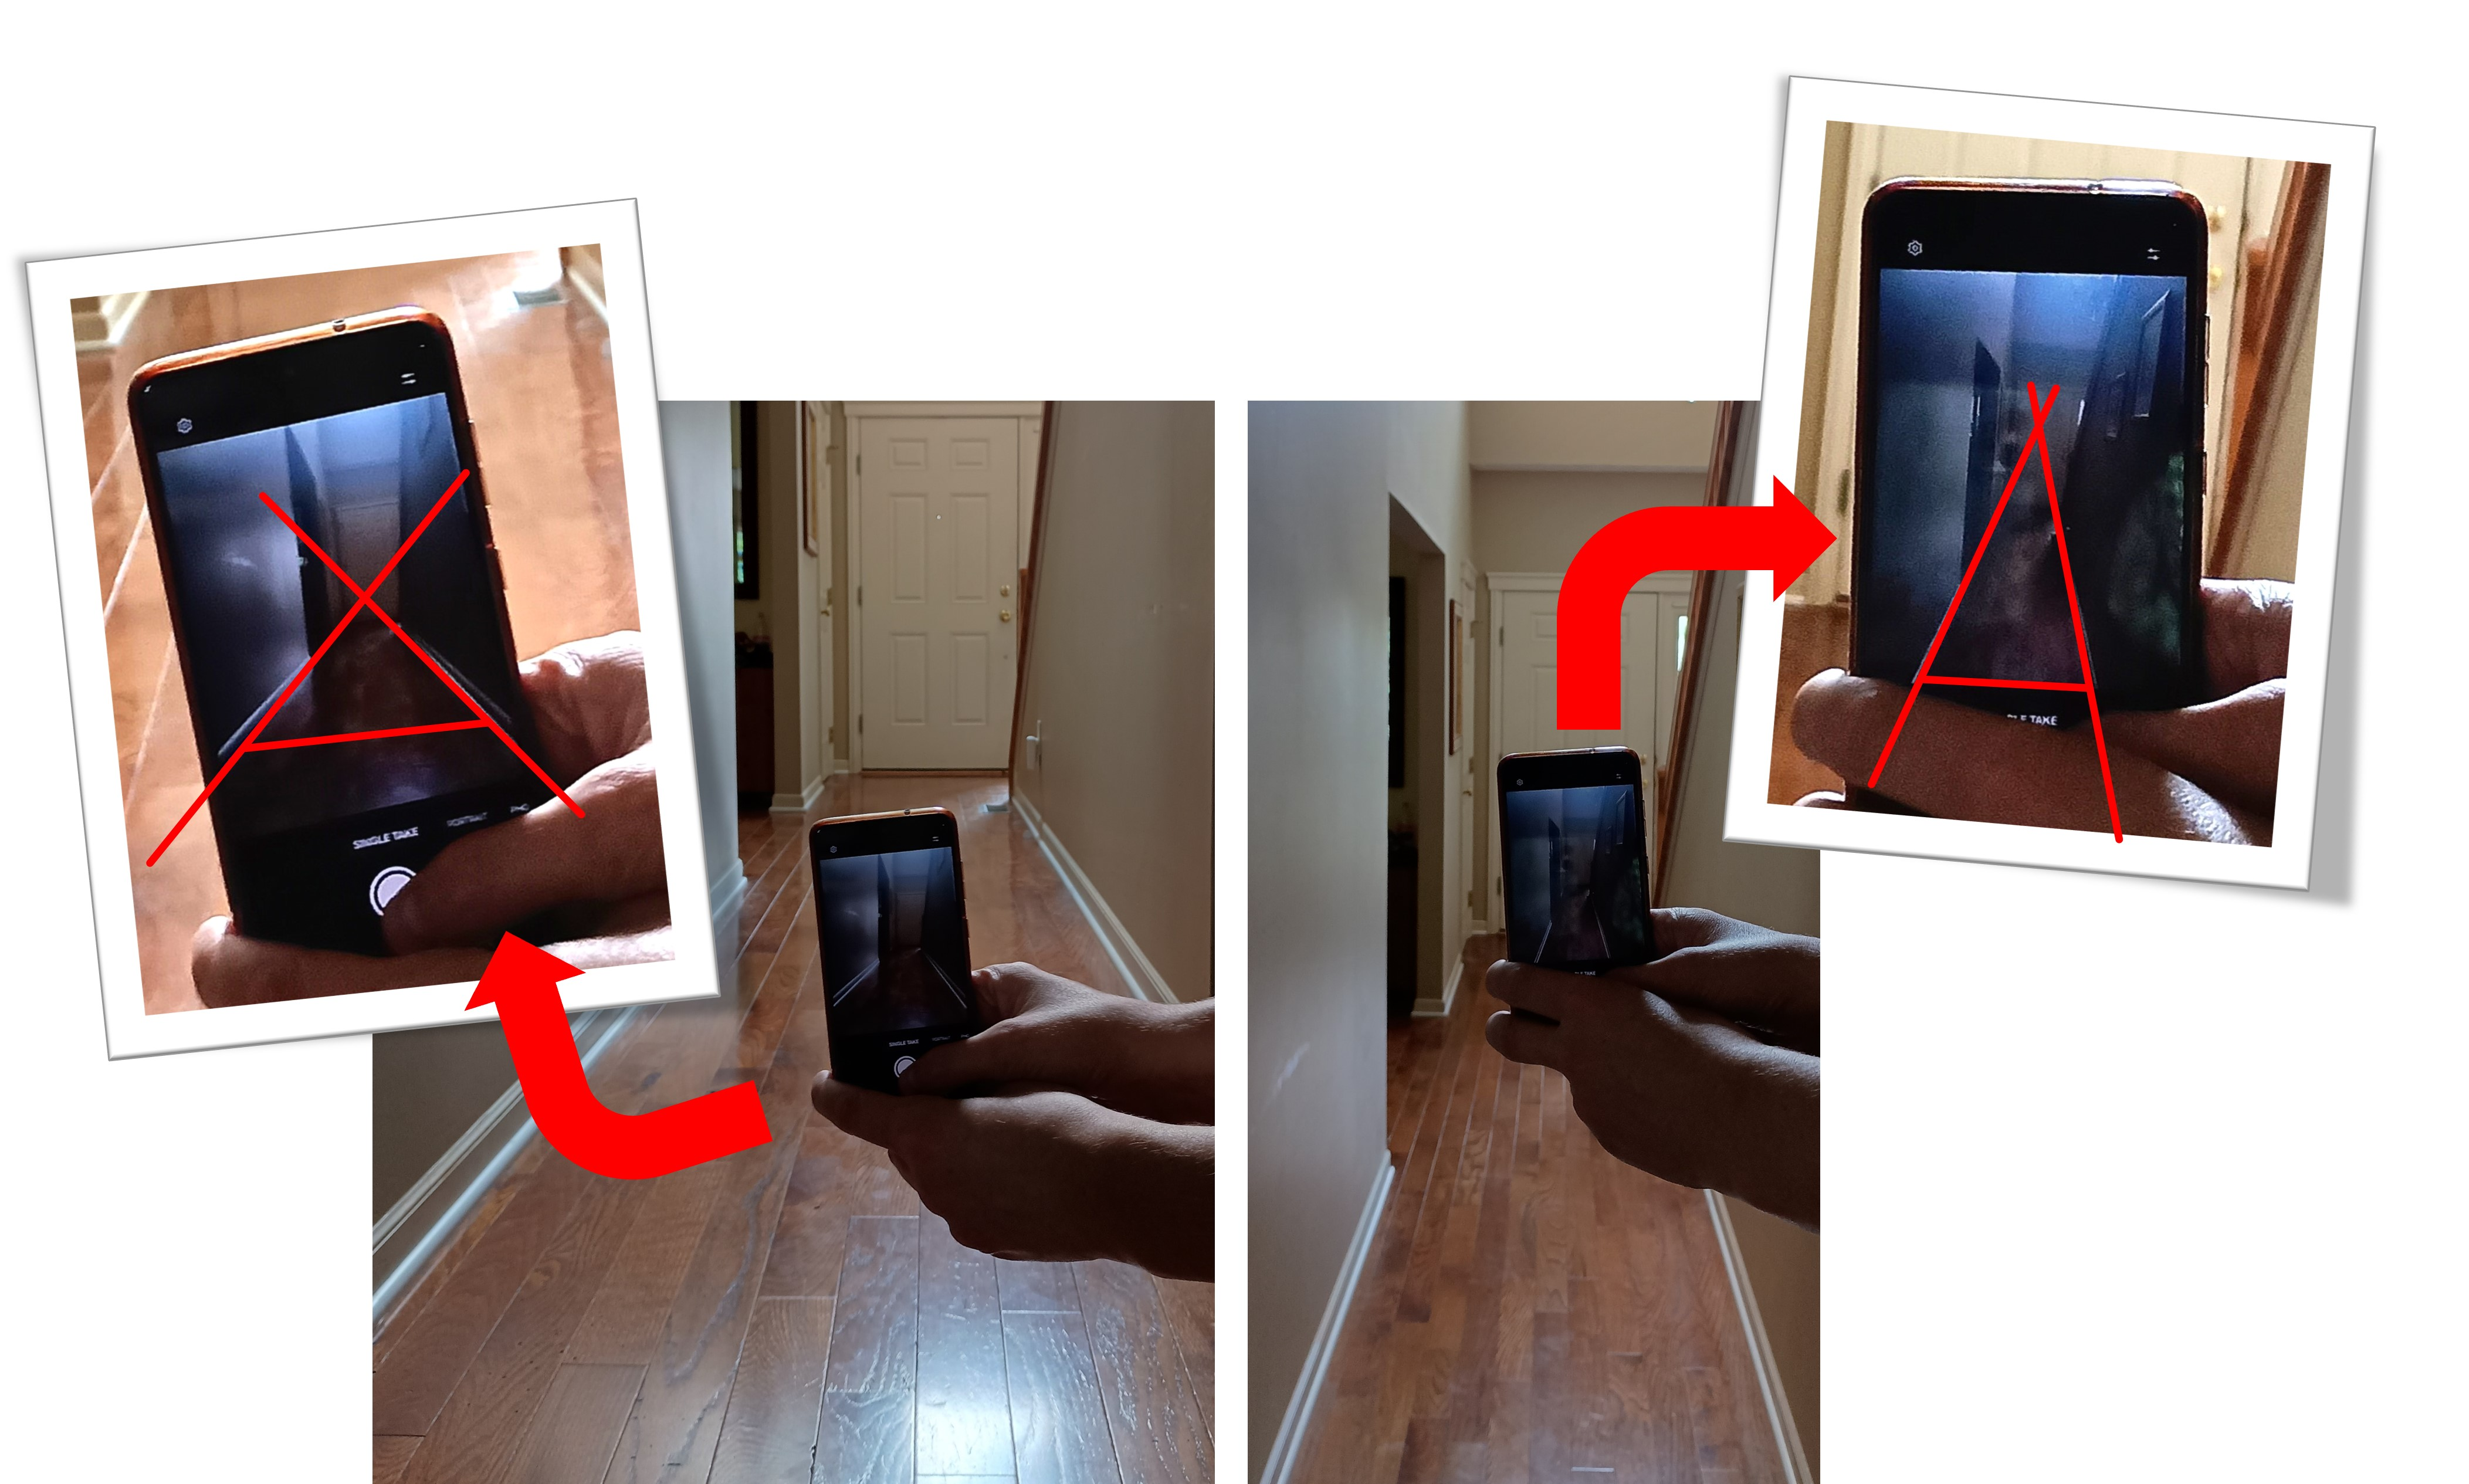
\includegraphics[width=6in]{doItYourself.jpg}
\end{image}

\begin{multipleChoice}
        \choice[correct]{As the camera lowers, the triangle becomes proportionally shorter.}
        \choice{As the camera lowers, the triangle becomes proportionally taller.}
        \choice{As the camera lowers, the triangle's proportions do not change.}
    \end{multipleChoice}

\end{exploration}

So far, we have established that there is a relationship between the proportions of the triangle formed by rails (or edges of a hallway), and the location of the camera that took the photo.  Next, we will look at a photo for which the measurements of the location and the position of the camera are known, and numerically relate the proportions of the triangle to the height of the camera.

\begin{exploration}\label{exp:hallway}
% In this exploration, we will use a photo 
% In groups of two or three, use a phone to take photos of a long desk, a sheet of paper or a hallway holding your phone at different heights, as shown below.


% To keep track of the camera height, we recommend that you hold or tape the phone to a meter stick or a ruler. Have one group member record the distance to the camera lens for every shot.  

% Import your shots into PowerPoint or OneNote.  Use the ruler tool (under ''Draw") to outline the edges of the hallway in each photo. Form a triangle with the vanishing point as the top vertex, as shown below.
The following photo shows a $92$-inch wide hallway.  The photo was taken with the camera lens $20$ inches above the floor.

\begin{image}
         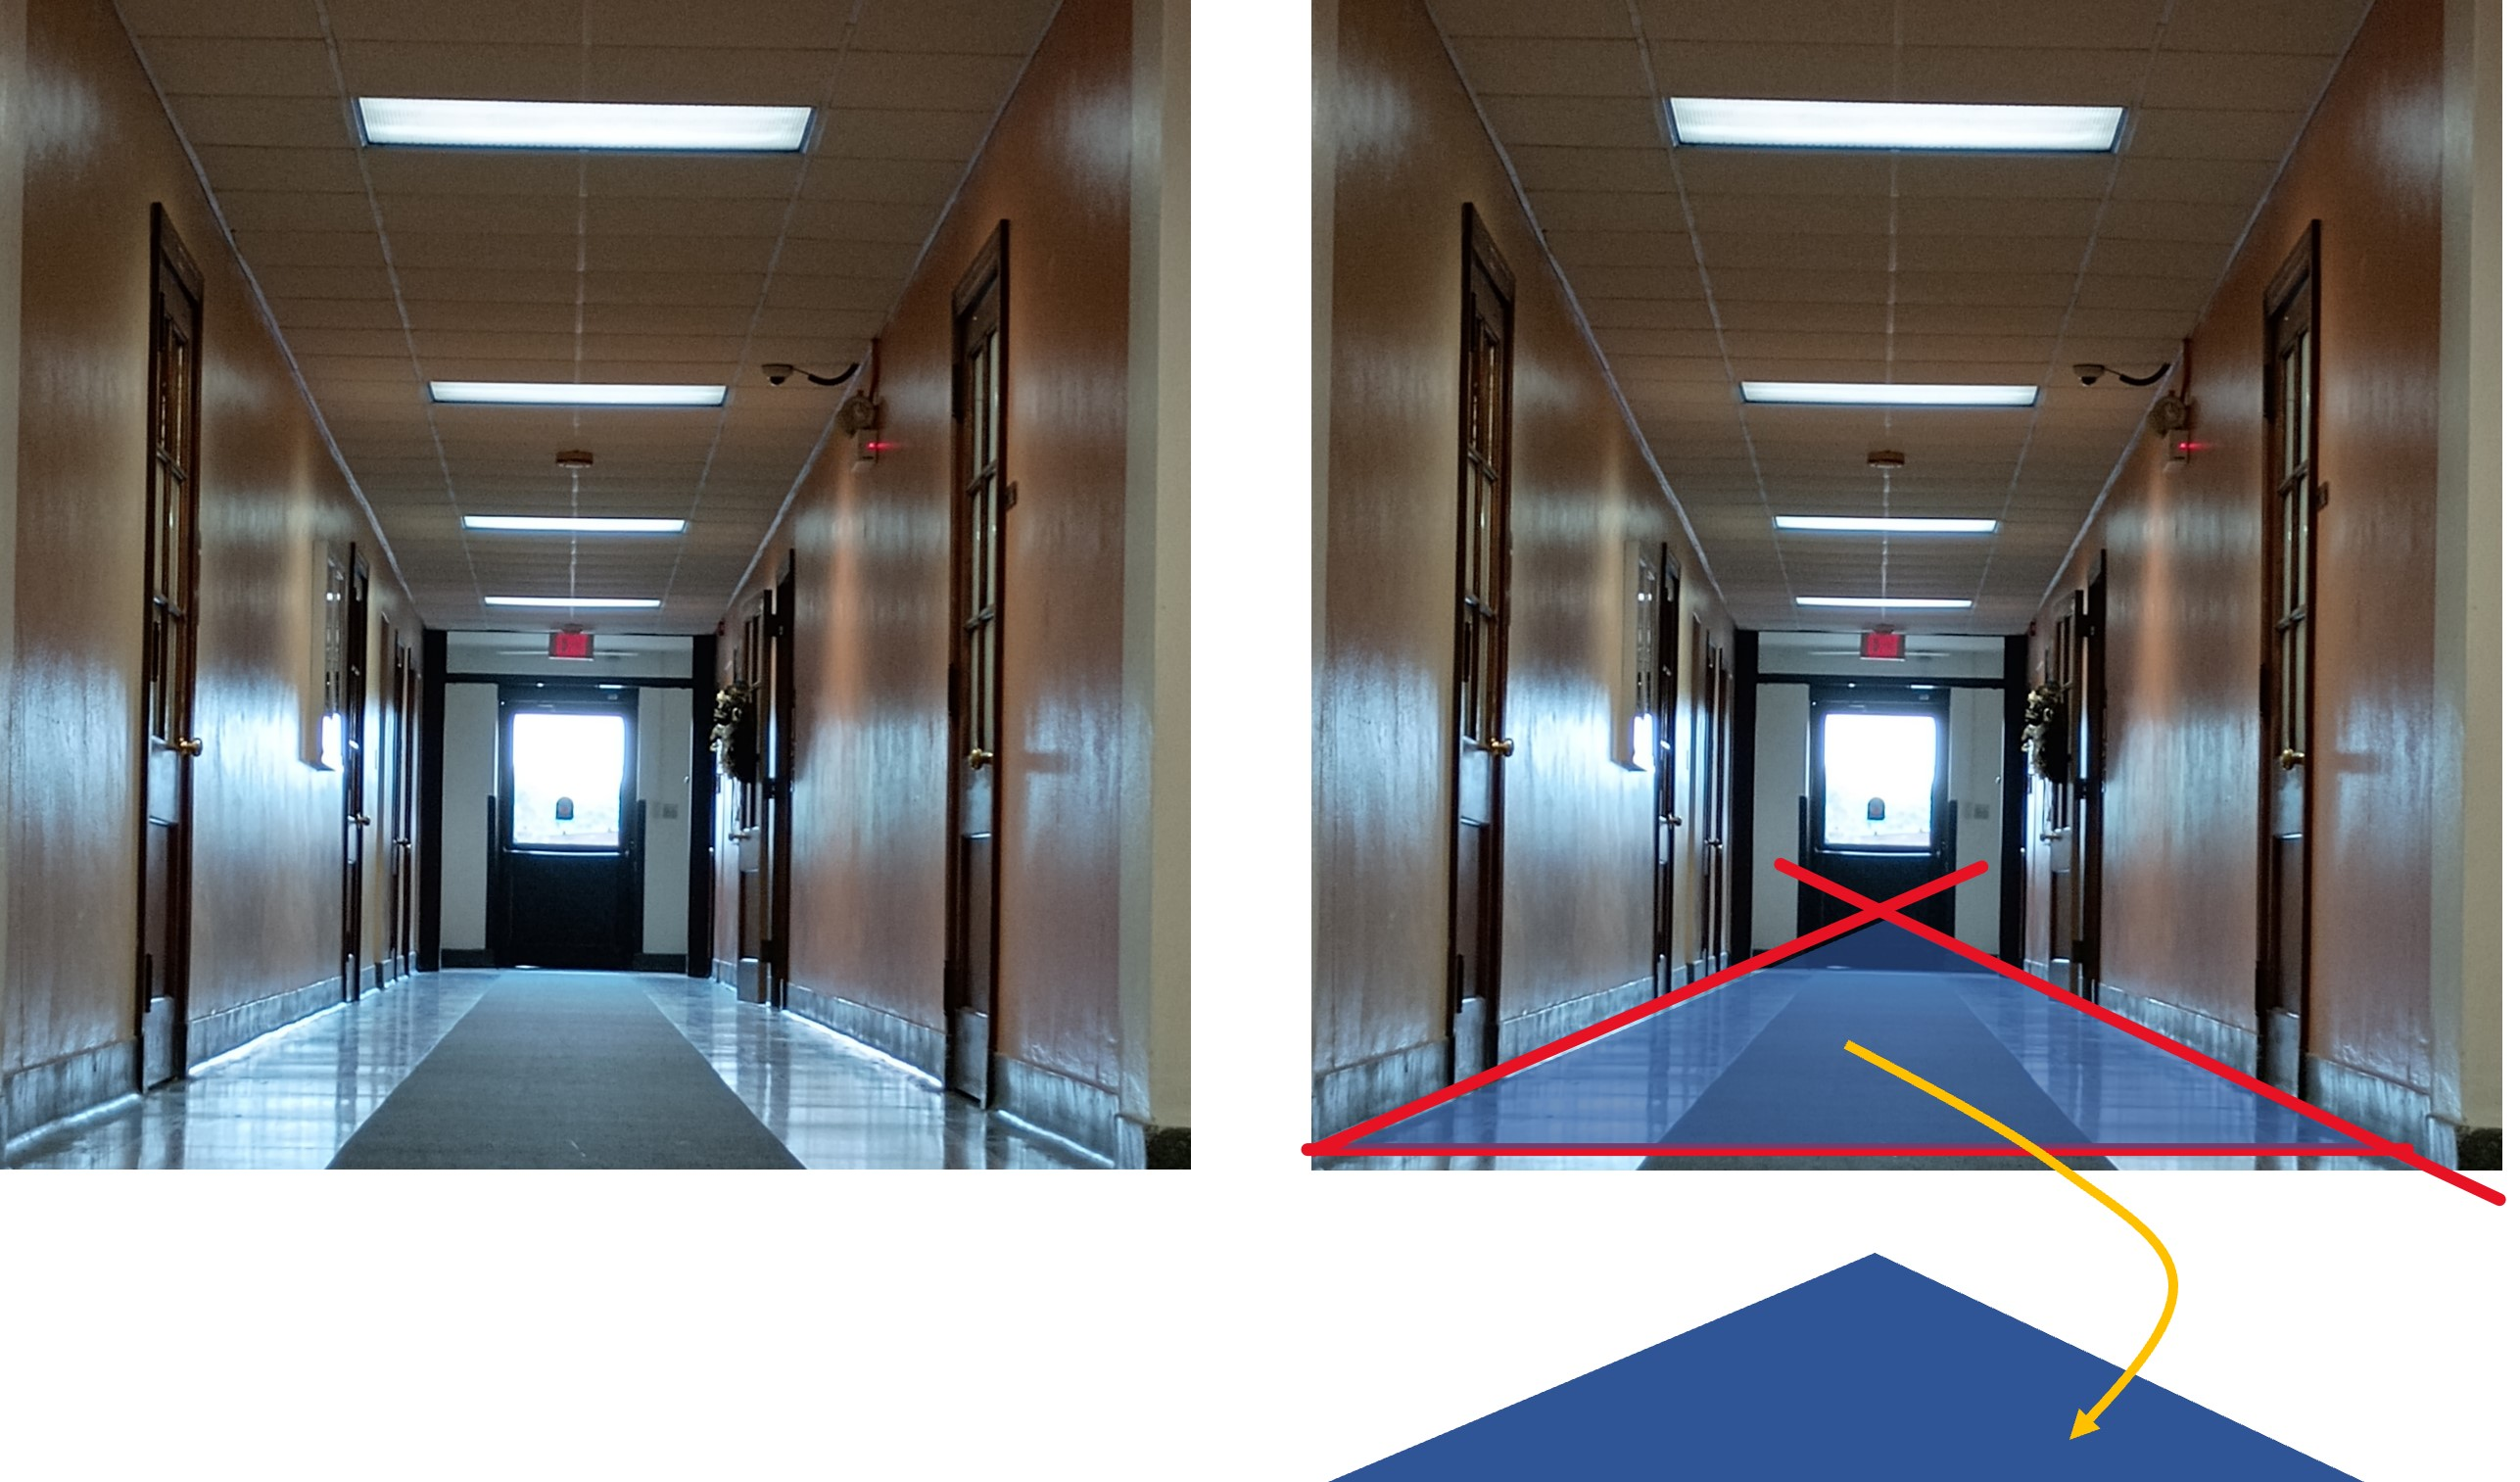
\includegraphics[width=5in]{hallwayExp.jpg}
\end{image}

% Observe that the triangle formed by the edges of the hallway is nearly isosceles.  This will be important for our future computations.  If your triangles are not isosceles, take a few more pictures, making sure that your camera lens is in the middle of the hallway (desk).

Observe that the resulting triangle is nearly isosceles.  We achieved this by placing the camera as close to the middle of the hallway as we could.  

We will now look at the ratio of the height of the triangle to the length of the base.
$$\frac{\text{height}}{\text{base}}=\frac{1.65}{7.5}=0.22$$

\begin{image}
         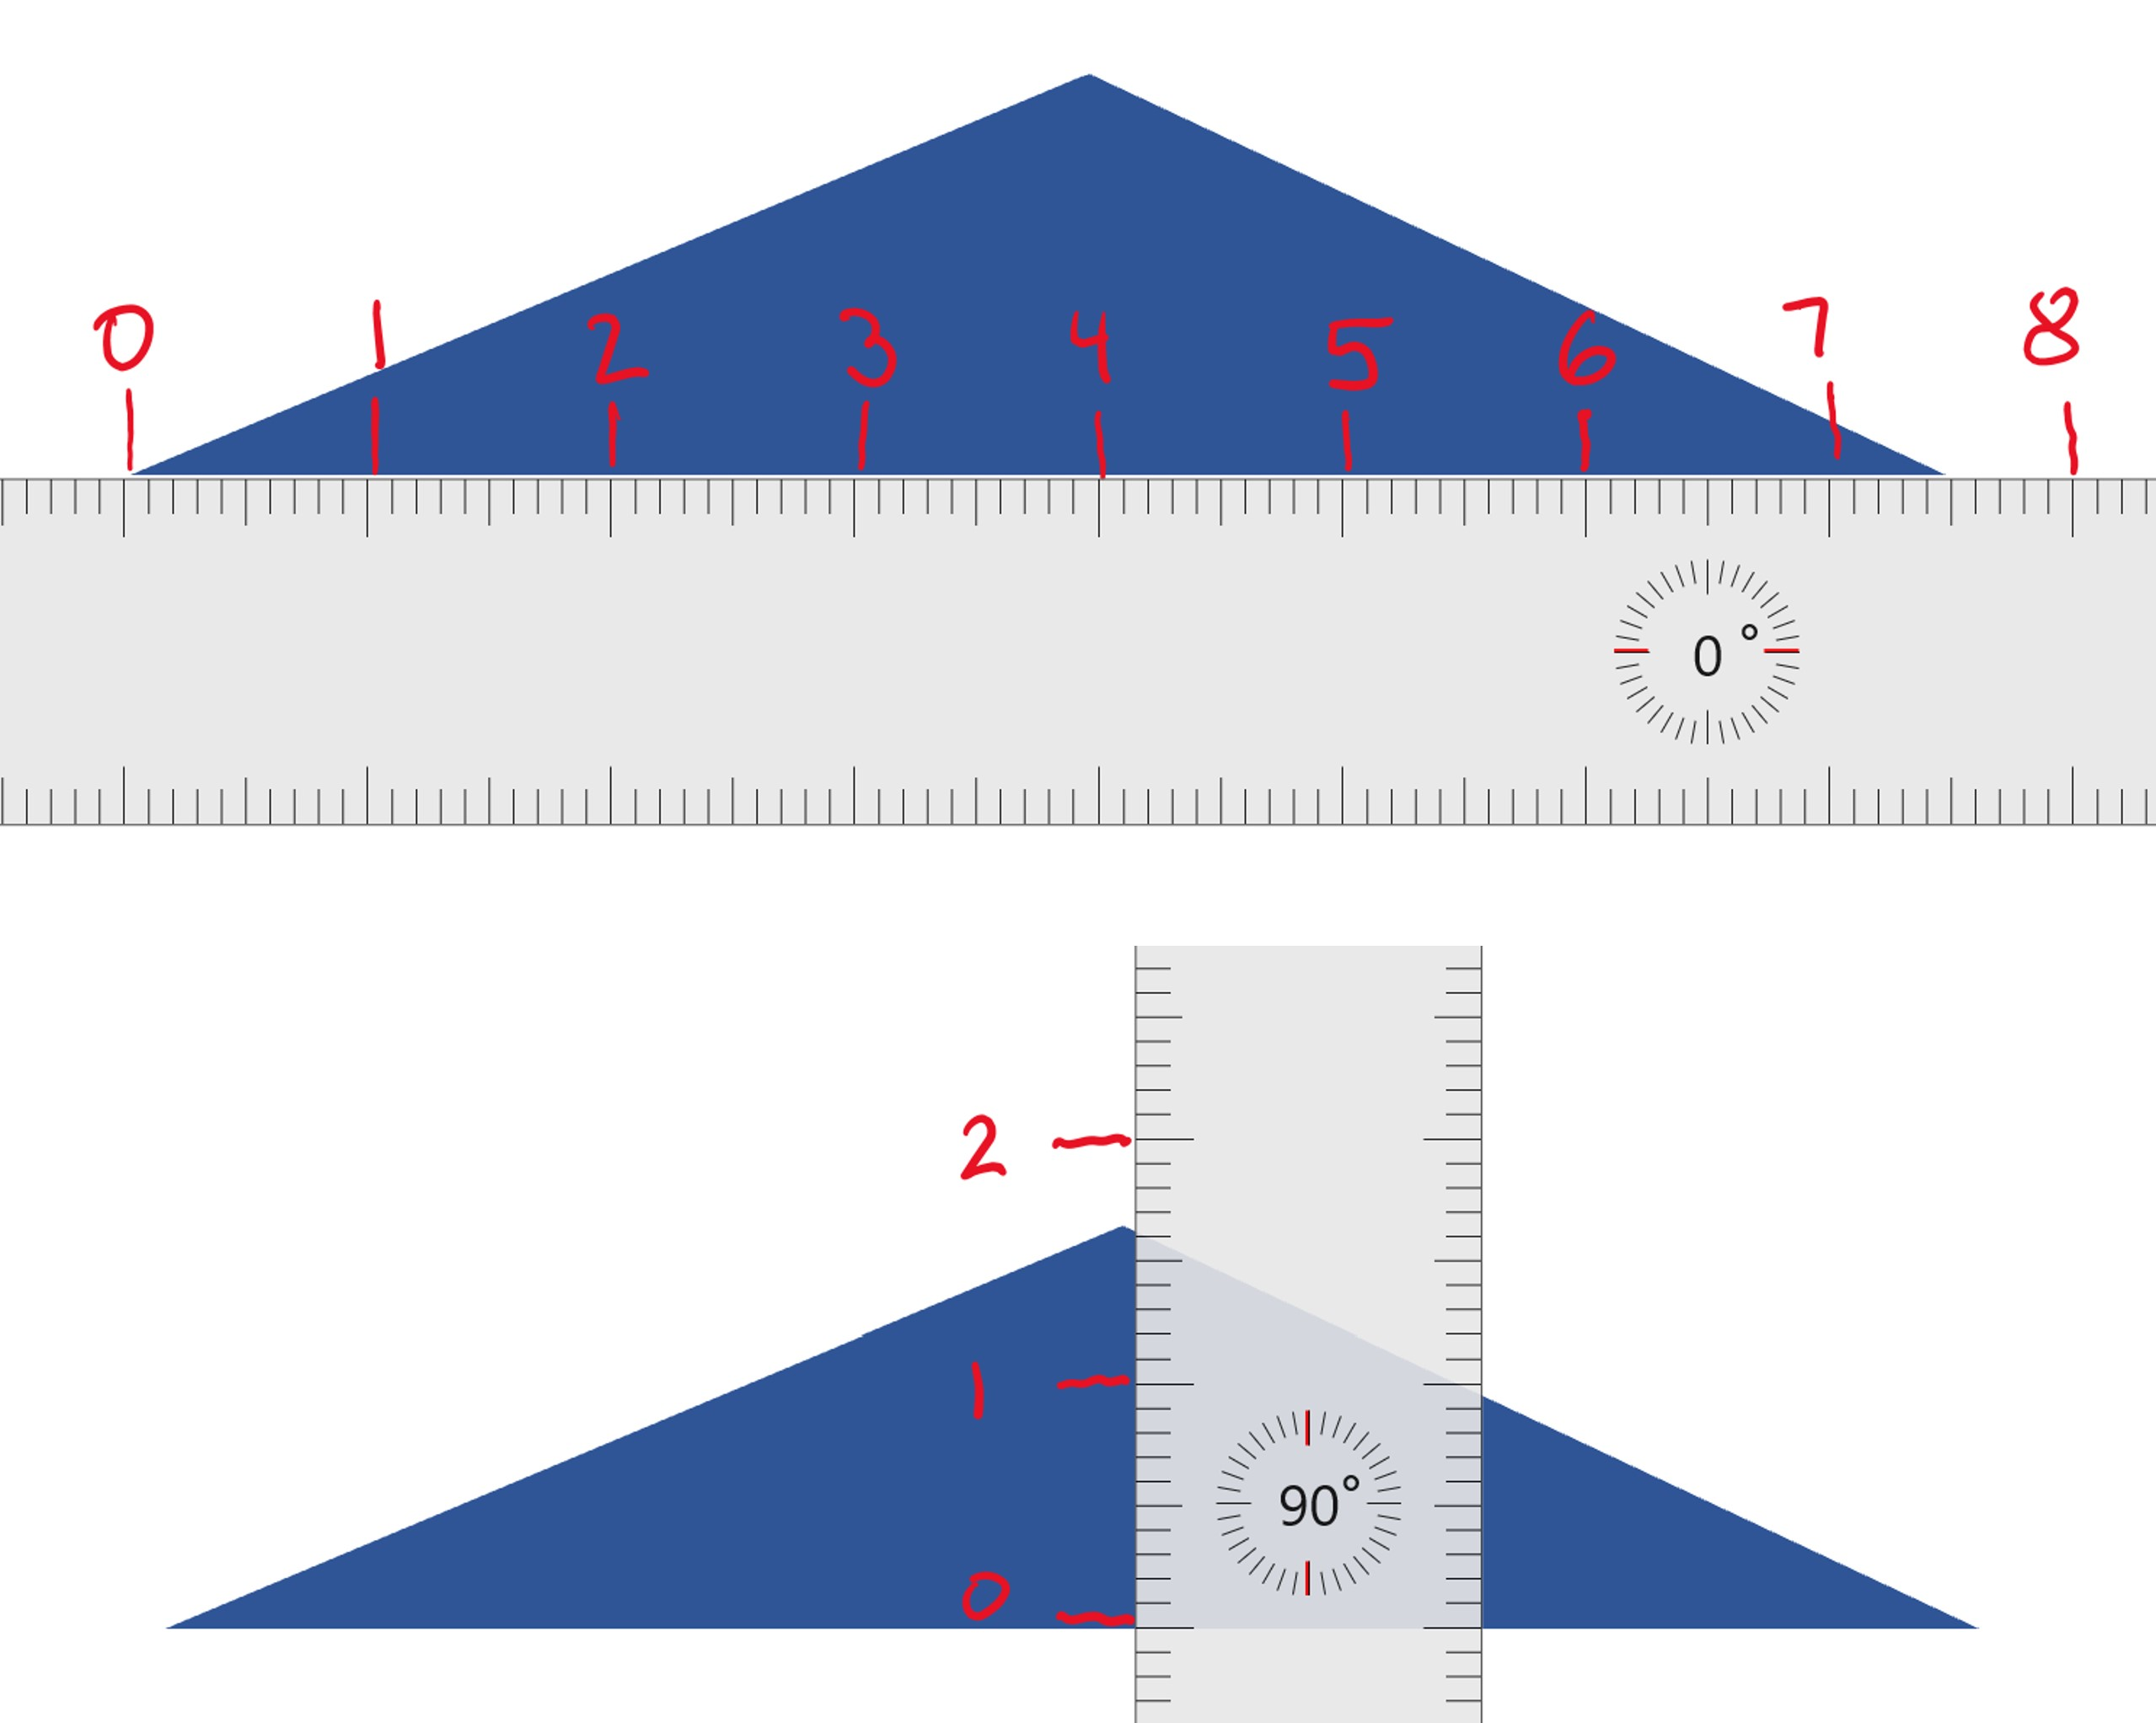
\includegraphics[width=4.5in]{triangleMeasures1.jpg}
\end{image}

\begin{question}
    Note that our calculations omitted the units.  Do units matter in this case?  If we were to do our measurements using different units, would the ratio still be the same? 
\end{question} 

Next, we will try to figure out what to do with this ratio to find an estimate for the height of the camera.  To do this, suppose we made four prints of our photo.  The first print is the size of a small poster, the last print is life-sized.  The resulting triangles are clearly of different sizes, but they have the same \emph{proportions}!  Such triangles are called \wordChoice{\choice{congruent} \choice{equilateral} \choice[correct]{similar}\choice{obtuse}}

\begin{image}
         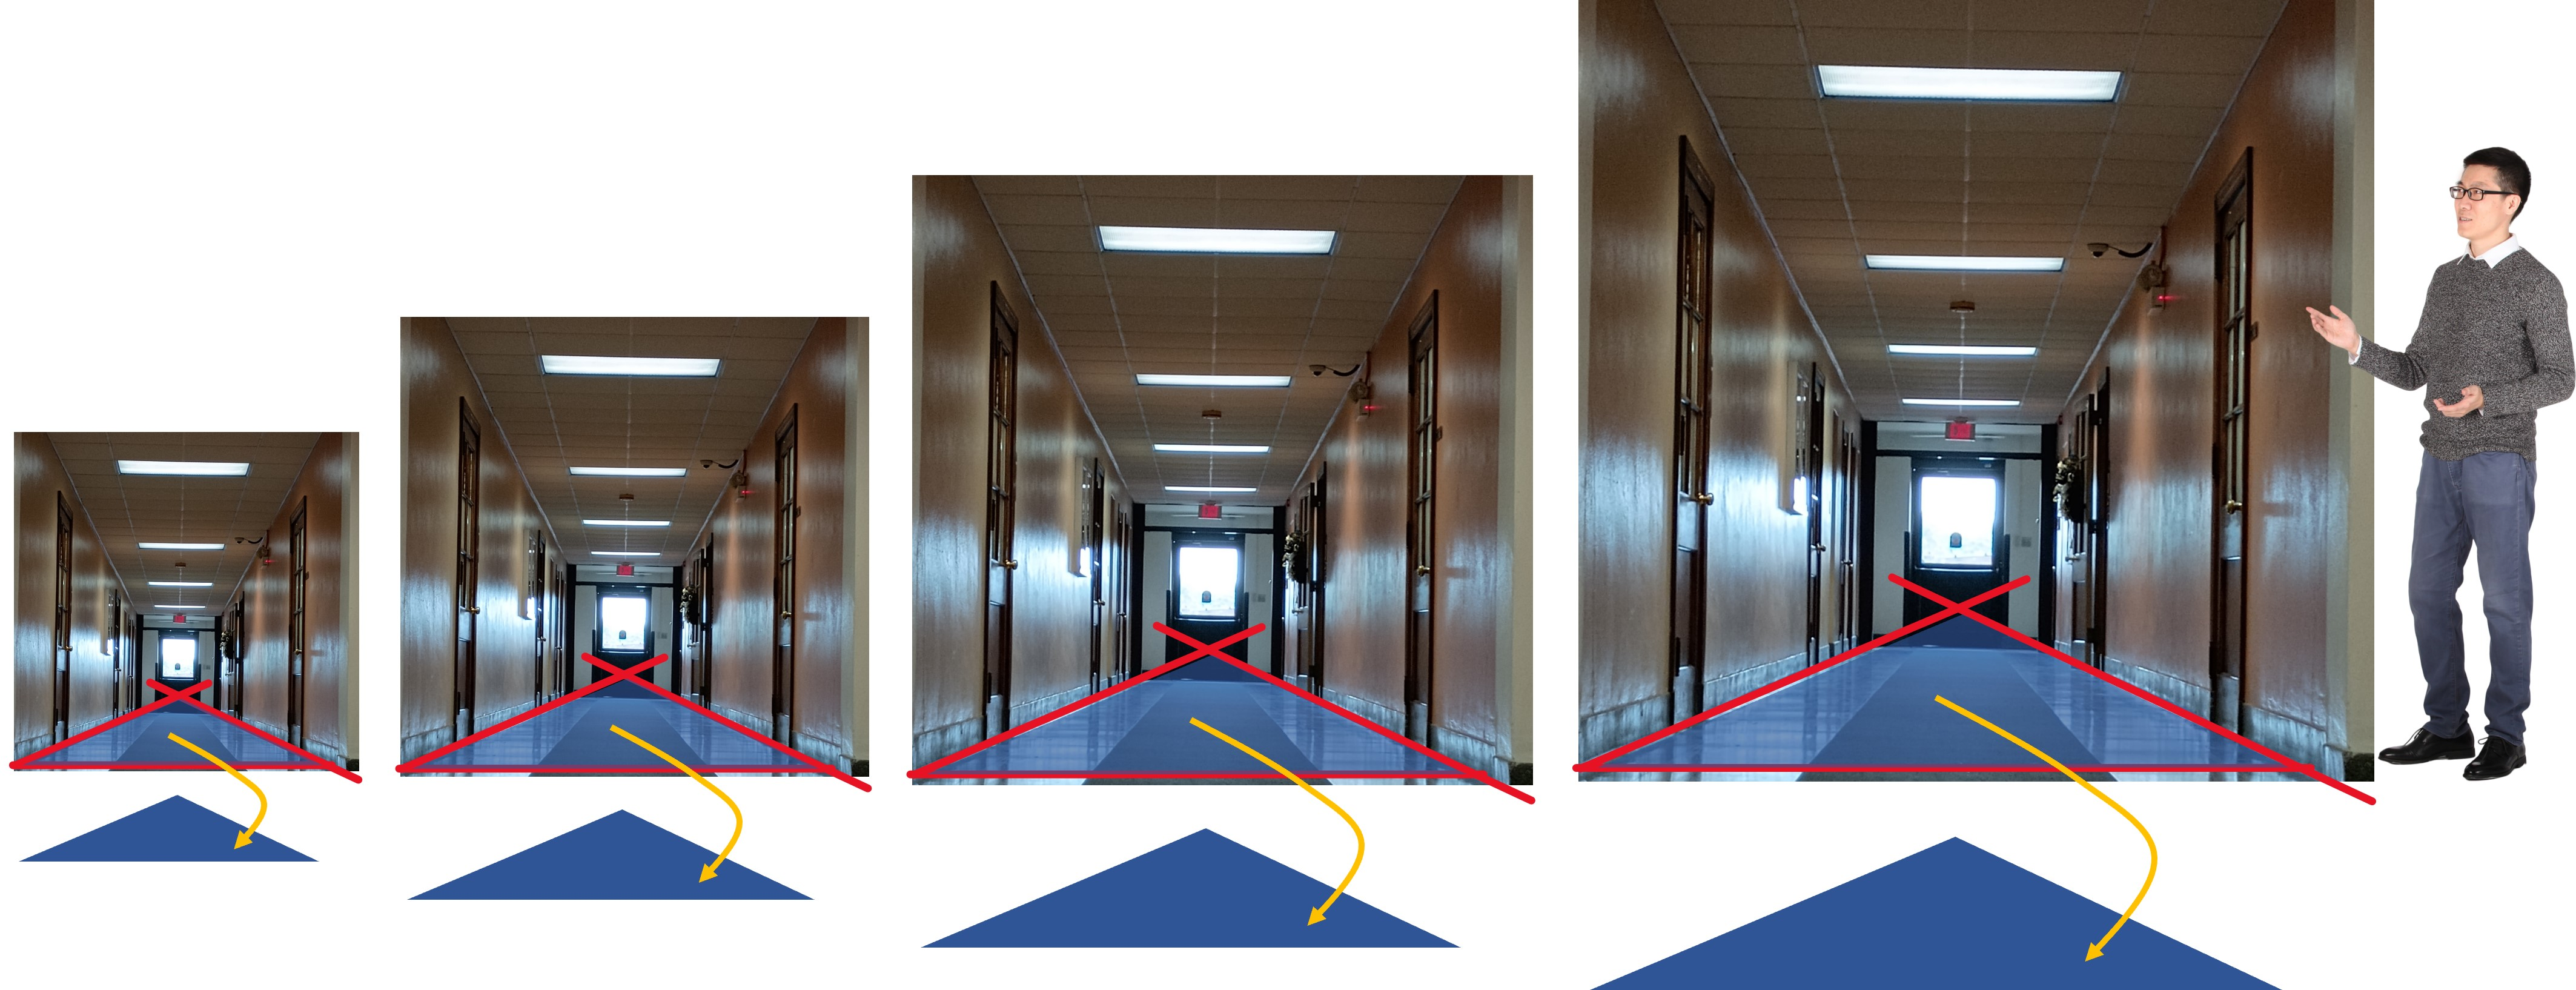
\includegraphics[width=5in]{similarHallways.jpg}
\end{image}

\begin{question}
    Since the last ''print" in the above graphic is life-sized, and the width of the real-life hallway is $92$ inches, we can conclude that the base of the last triangle is $92$ inches. 
    Set up and solve a proportion to find the height of the last blue triangle.  
    $$\frac{1.65}{7.5}=0.22=\frac{\text{height of last triangle in inches}}{\answer{92}\text{in}}$$
    $$\text{Height of last triangle}=\answer{20.24}$$

    Compare your answer to the height of the camera given at the start of the problem.  The numbers are very close!  Do you think this is a coincidence?  
\end{question}

\begin{question}
    The height of the camera above the floor was given to be $20$ inches, but the computed height of the triangle was not exactly $20$.  What do you think accounts for the difference?
\end{question}

\begin{question}
    Formulate a rule for finding the height of the camera for photos with the same set up.  How would you verify that your rule works for all such photos?  Discuss this with your classmates and your teacher.
\end{question}
\end{exploration}




\end{document}